\documentclass{article}
\usepackage[utf8]{inputenc}
\usepackage{graphicx}



\title{Membuat Aplikasi Di Apex Melalui Excel}
\author{Yusuf Jordan El Anwar }
\date{October 2019}

\begin{document}

\maketitle

\section{ Cara Pembuatan Aplikasi}

\begin{enumerate}
    \item Sebelum membuatan aplikasi baru di apex online melalui excel. Kita harus membuat data di excel. Disini saya memiliki Data Mahasiswa D3TI. Dan Data tersebut akan saya coba jadikan Aplikasi melalui Apex.  
    \begin{center}
         \centering
            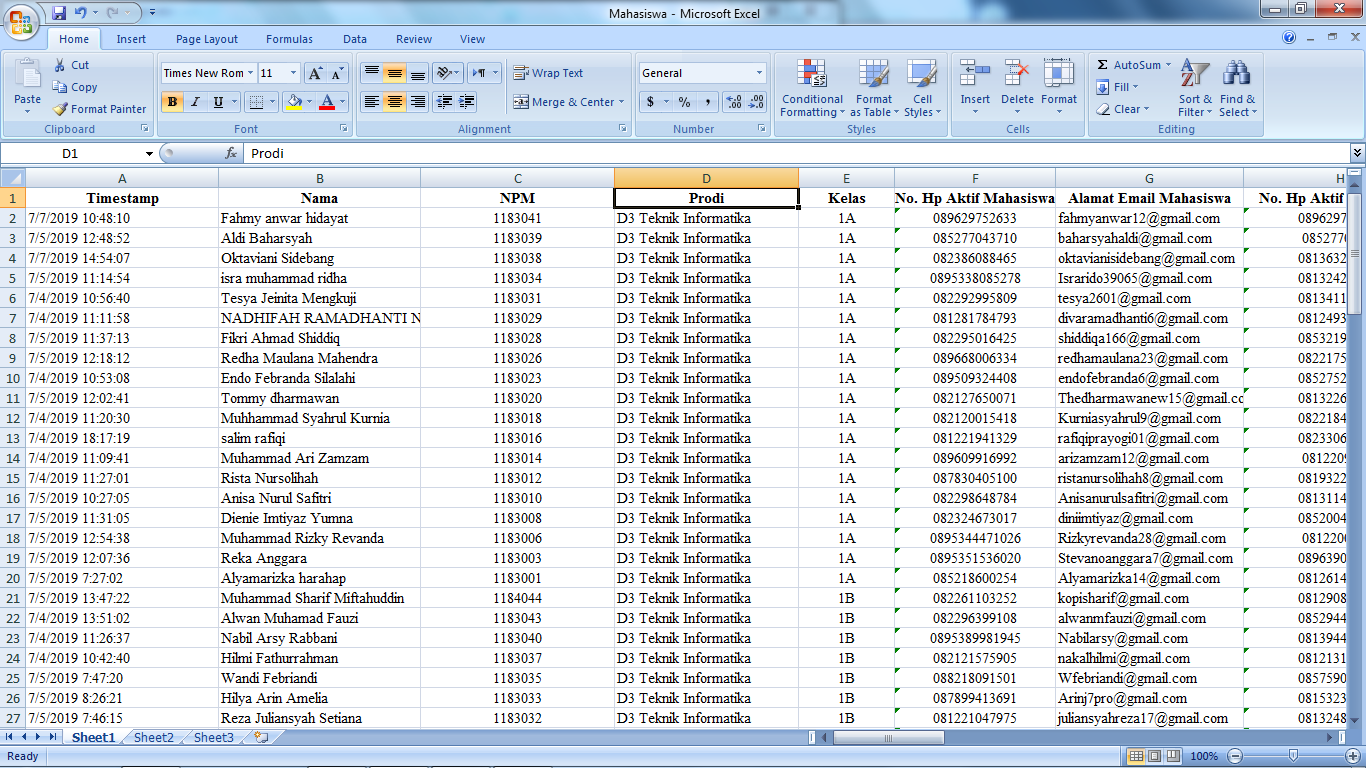
\includegraphics[scale=0.27]{figures/DB0.png}
        \caption{Menambahkan Data}
        \label{excel}
    \end{center}
       
     \item langkah selanjutnya buka di browser apex oracle online kemudian login. Setelah masuk dashboard pilih App builder lalu pilih create
    \begin{center}
         \centering
            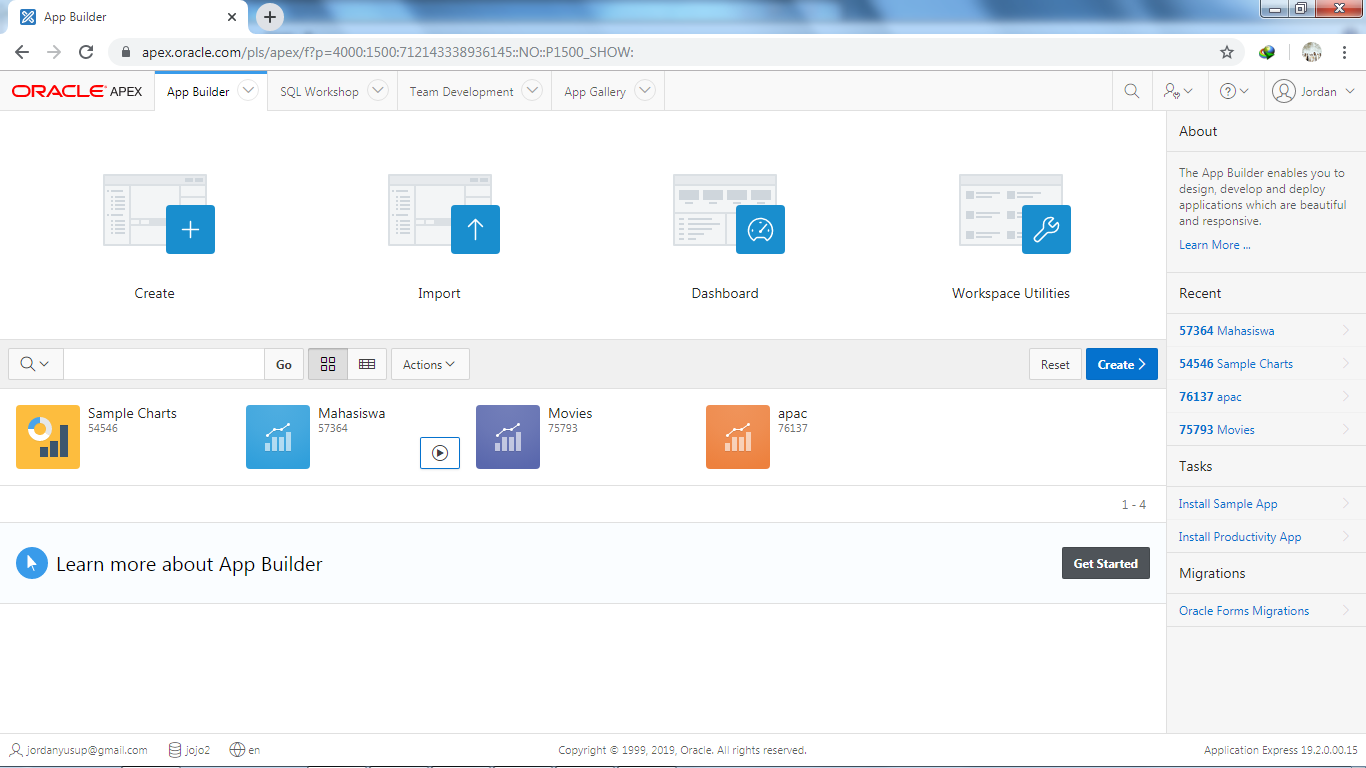
\includegraphics[scale=0.27]{figures/DB1.png}
        \caption{create aplikasi}
        \label{create}
    \end{center}
    
      \item Kemudian kita akan diberi pilihan untuk membuat aplikasi baru, membuat aplikasi dari file, dan melakukan instalasi aplikasi yang disediakan oracle. Kita pilih Form a File.
    \begin{center}
         \centering
            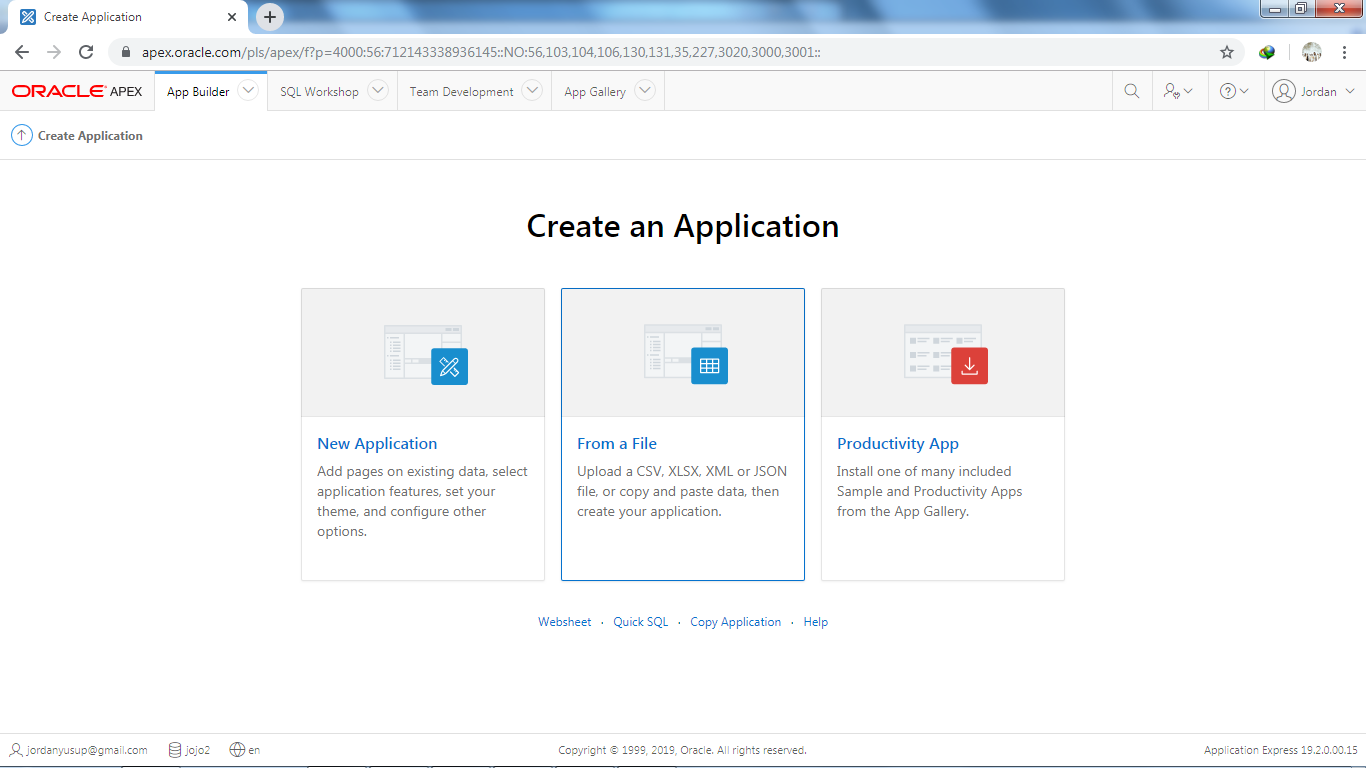
\includegraphics[scale=0.27]{figures/DB2.png}
        \caption{chosse a file}
        \label{from}
    \end{center}
    
    \item Selanjutnya sistem akan menampilkan tampilan load file. Disini kita dapat mendrop file maupun mencopy paste data di excel yang tadi dibuat. Disini saya mendrop file excel mahasiswa. 
    \begin{center}
         \centering
            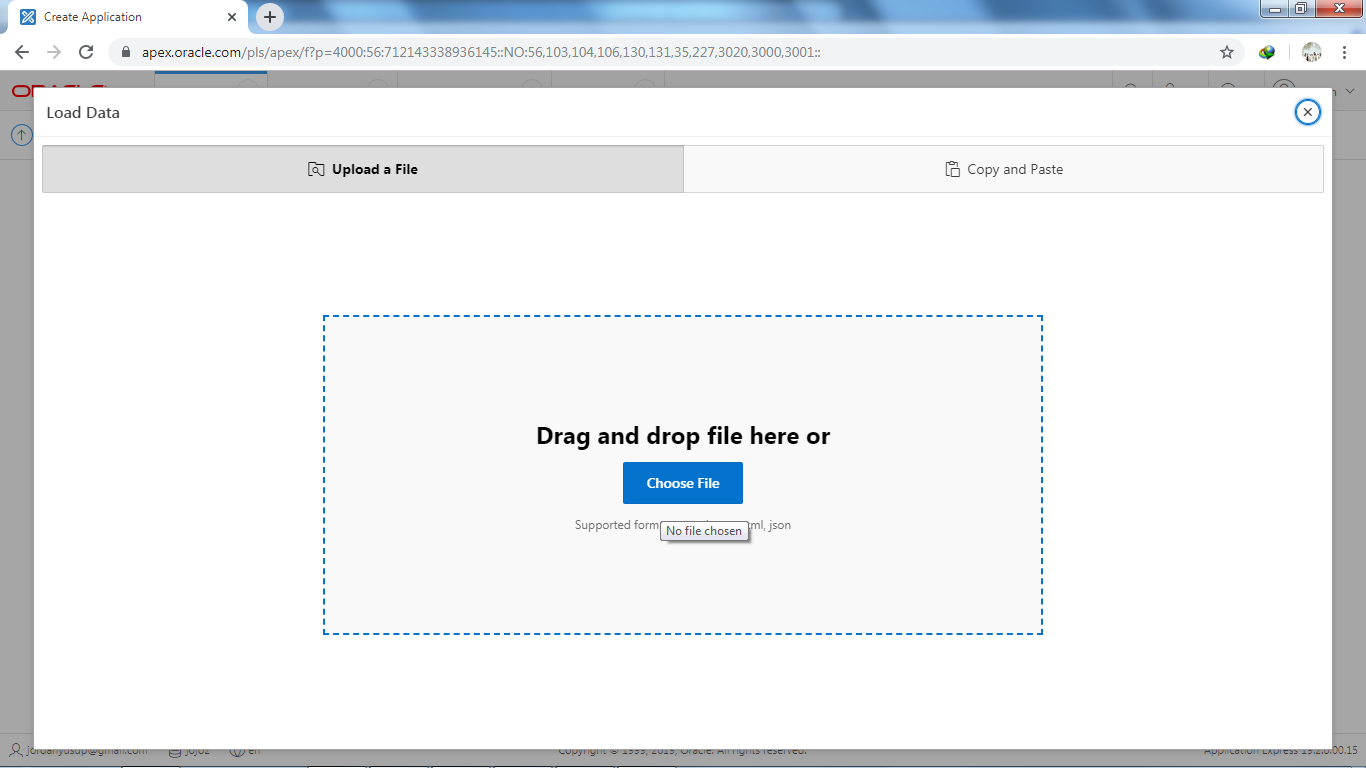
\includegraphics[scale=0.27]{figures/DB3.png}
        \caption{LOAD DATA}
        \label{chosse}
    \end{center}
    
    \item Karena sebelumnya saya telah memiliki aplikasi bernama mahasiswa saya membuat nama Mahasiswa D3TI 
    \begin{center}
         \centering
            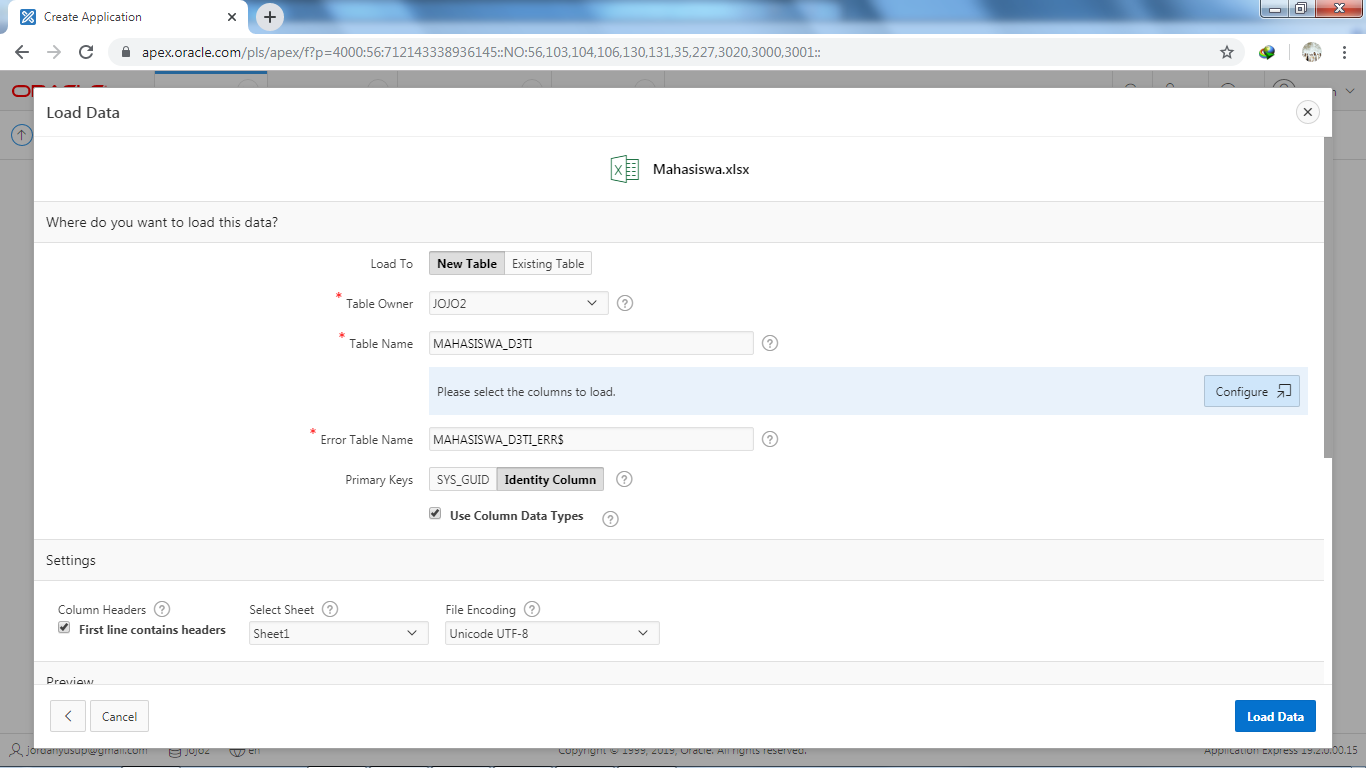
\includegraphics[scale=0.27]{figures/DB4.png}
        \caption{Drag & Drop}
        \label{excel}
    \end{center}
    
    \item klik create aplications 
    \begin{center}
         \centering
            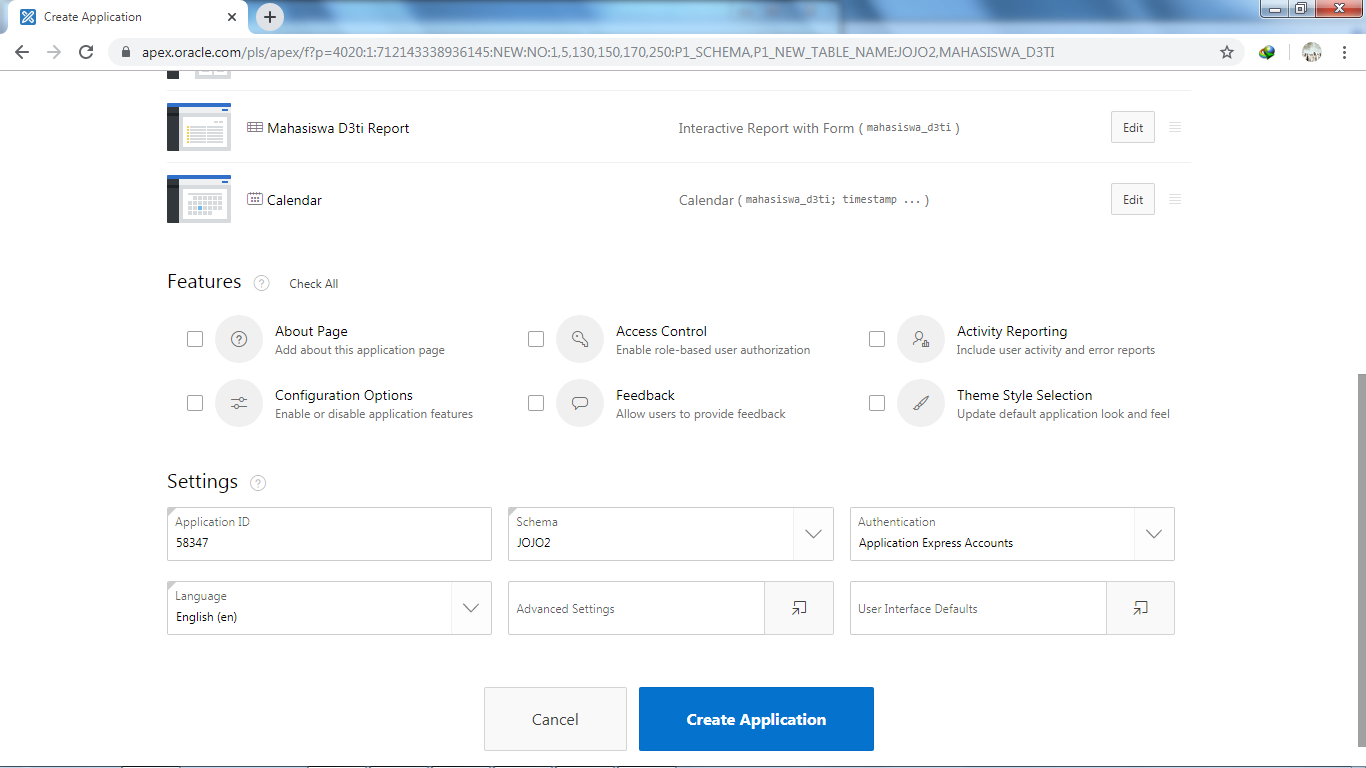
\includegraphics[scale=0.27]{figures/DB5.png}
        \caption{proses create aplication}
        \label{excel}
    \end{center}
    
    \item run aplication untuk menjalankan Aplikasi yang telah dibuat
    \begin{center}
         \centering
            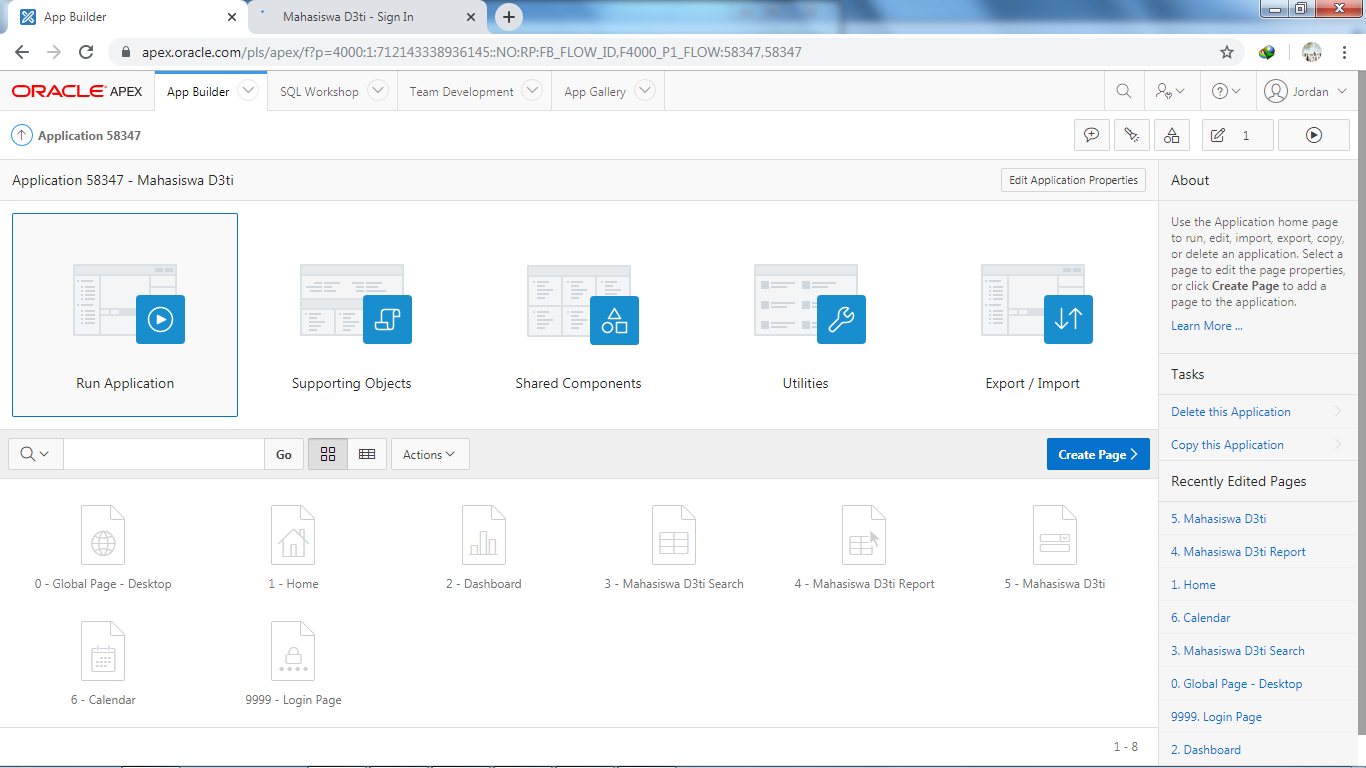
\includegraphics[scale=0.27]{figures/DB6.png}
        \caption{run aplication}
        \label{excel}
    \end{center}
    
    \item Kemudian Kita akan kembali login setelah itu muncul tampilan dari Aplikasi yang telah di buat. 
     
    \begin{center}
         \centering
            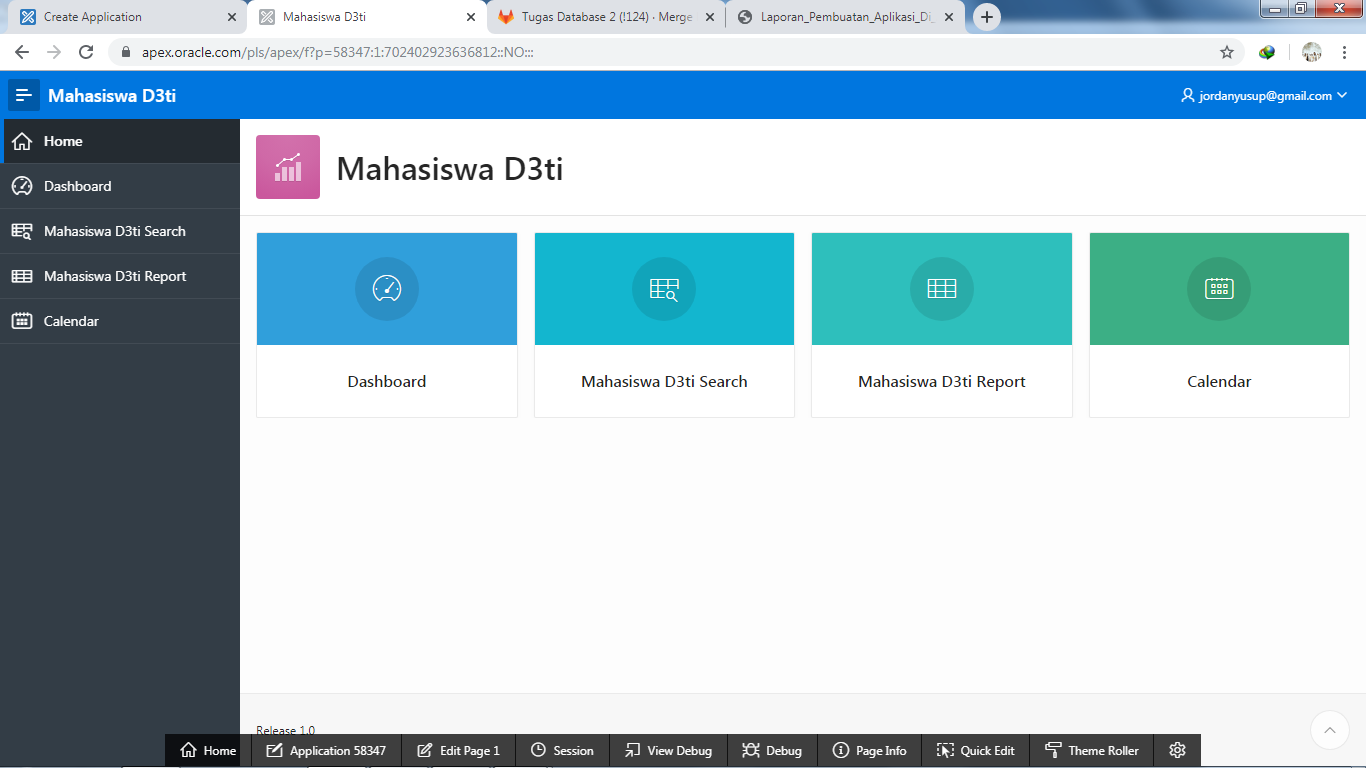
\includegraphics[scale=0.27]{figures/DB9.png}
        \caption{Tampilan Aplikasi}
        \label{excel}
    \end{center}
        
    \item Pilih Menu Mahasiswa D3TI Report Klik Action Pilih Chart
    \begin{center}
         \centering
            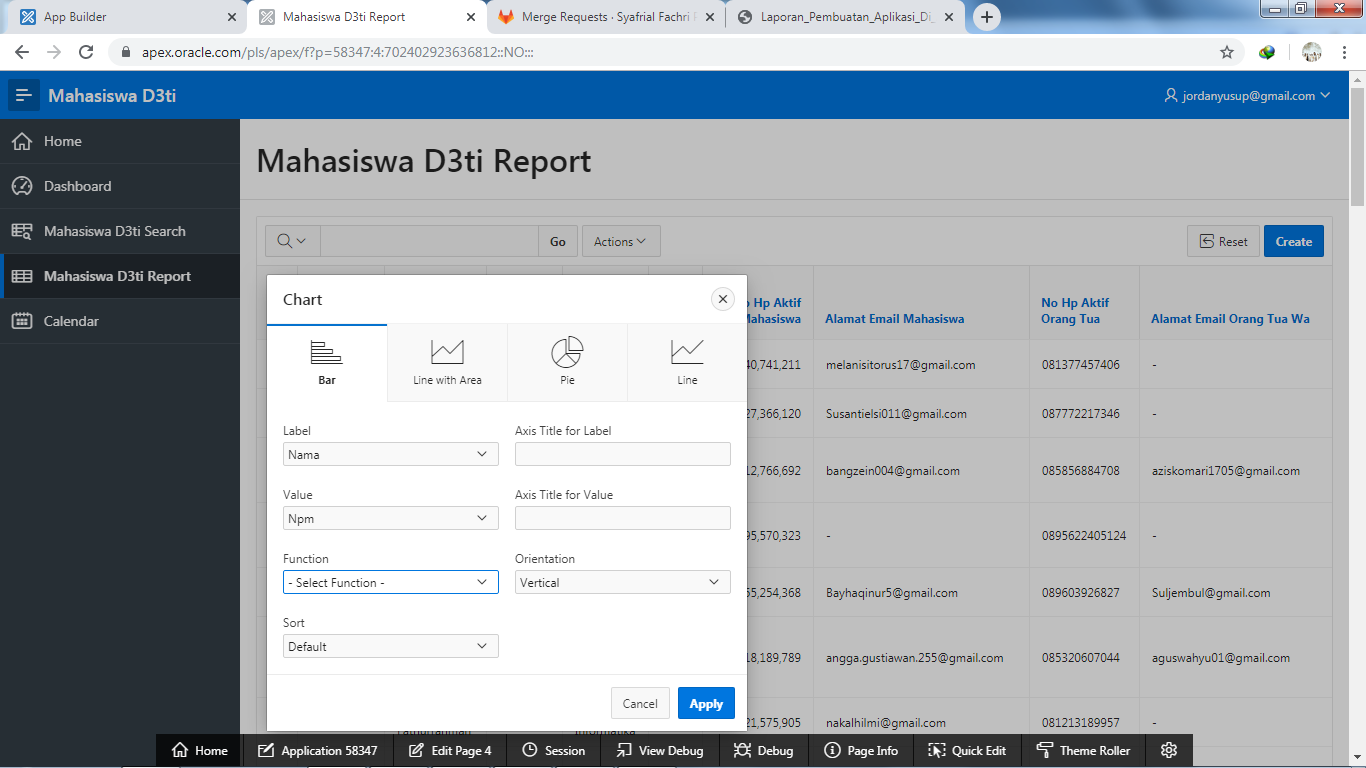
\includegraphics[scale=0.27]{figures/DB7.png}
        \caption{D3TI Report}
        \label{excel}
    \end{center}
    
    \item Pilih Chart yang Di inginkan.
    \begin{center}
         \centering
            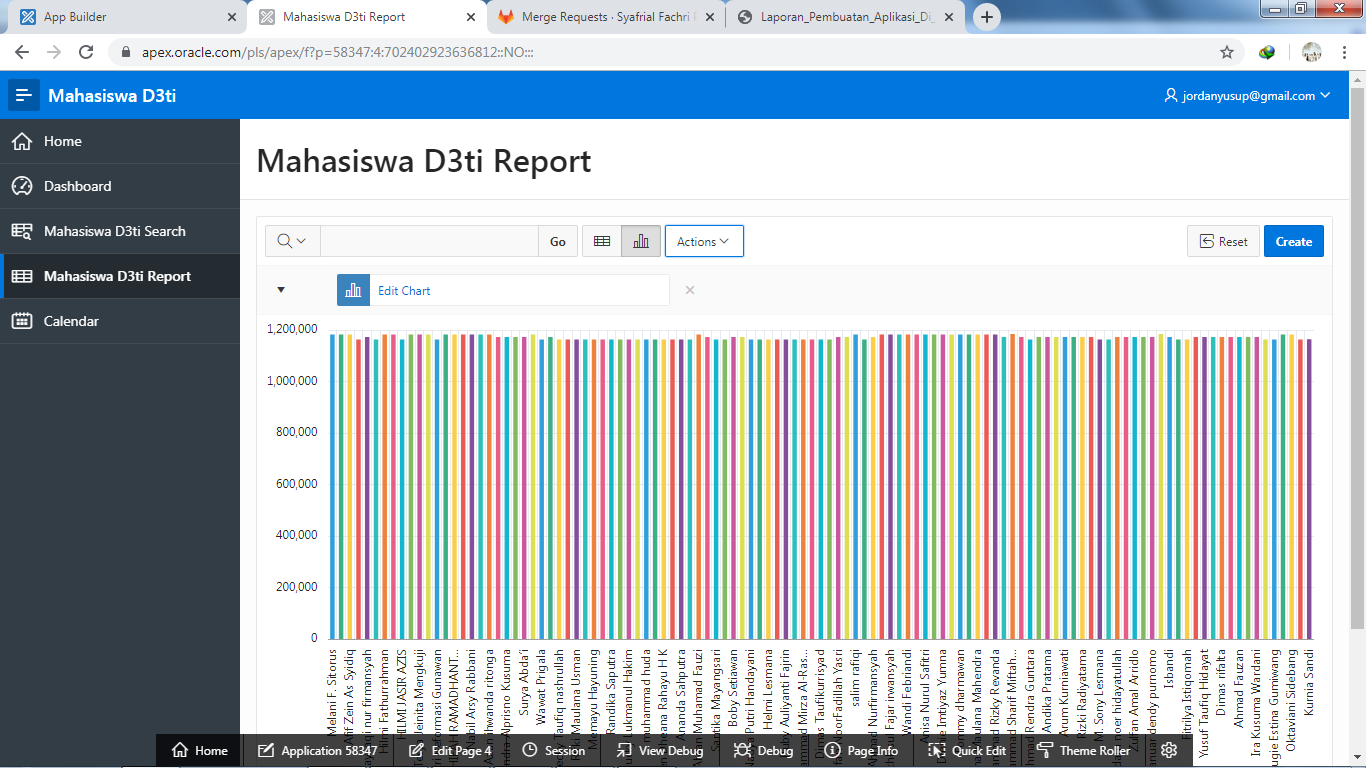
\includegraphics[scale=0.27]{figures/DB8.png}
        \caption{Tampilan Aplikasi}
        \label{excel}
    \end{center}            
       
\end{enumerate}



\section{Password username}
          \item workspace "JOJO2"
          
          \item username "jordanyusup@gmail.com"
          
          \item password "J012d4nb4"
      
      
       
\end{document}
